%!TEX TS-program = xelatex
%!TEX encoding = UTF-8 Unicode
%!TeX spellcheck = it_IT
%!TEX root = ../tesi.tex

\chapter{Modello a ostacoli}\label{chap:modello-a-ostacoli}
%
\section{Il modello matematico}\label{sec:il-modello-matematico}
Il modello utilizzato viene descritto per la prima volta in~\cite{5720204}, dove viene presentato
come un'estensione dei cosiddétti modelli di attenuazione del segnale.
In generale, questi possono essere scritti nella forma dell'Equazione~\ref{eq:fading-models}, dove $P$ è la potenza del trasmettitore (e ricevitore),
$G$ i guadagni delle antenne e $L$ il termine che indica le attenuazioni dovute alla trasmissione.
%
\begin{gather}
	P_r[dBm] = P_t[dBm] + G_t[dB] + G_r[dB] - \sum L_x[dB] 														\label{eq:fading-models} \\
	L_{TwoRayGround} = 10 \lg \left( \frac{d^4 L}{h^2_t h^2_t} \right)	\qquad [dB]		\label{eq:tworayground-model} \\
	L_{LogNorm} = 10 \lg \left( X_\sigma \right)	\qquad [dB]													\label{eq:lognorm-model}
\end{gather}
%
Questi modelli possono essere espressi come componenti di $L$ e concatenati in modo da ottenere l'attenuazione totale risultante.
Ad esempio, le equazioni~\ref{eq:tworayground-model} e~\ref{eq:lognorm-model} illustrano rispettivamente i modelli a doppio raggio e log-normale.

Il modello in esame rappresenta la perdita di segnale dovuta a un ostacolo estendendo l'Equazione~\ref{eq:fading-models}
col termine $L_{s,o}$, che unisce l'attenuazione causata dai bordi dell'ostacolo (attenuazione per-parete)
e quella derivante dalla superficie interna (attenuazione per-metro):
%
\begin{gather}\label{eq:osbtacle-model}
	L_{s,o} = \alpha n + \beta d_o
\end{gather}
dove $n$ è il numero di volte che il bordo dell'ostacolo viene intersecato dalla visuale e $d_o$ è la distanza, in metri, attraversata all'interno dell'ostacolo.
Il primo dei due parametri di calibrazione, $\alpha$, espresso in decibel per metro (dB/m), descrive l'attenuazione
che la trasmissione subisce a causa delle pareti esterne dell'ostacoli.
Il secondo, $\alpha$, espresso in decibel (dB per parete), serve come misura di approssimare della struttura interna dell'ostacolo.
Tramite la regolazione di questo valore è possibile rappresentare diverse tipologie di ostacoli.

Prendendo il caso di edifici in un ambiente cittadino, i valori predefiniti per i due parametri sono $\alpha = 9$ dB per parete e $\beta = 0,4$ dB/m.
%
\begin{figure}[htbp]
	\centering
		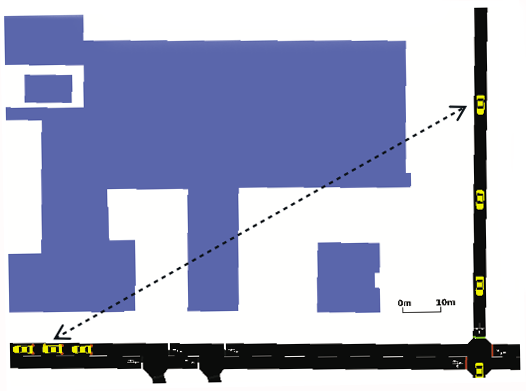
\includegraphics[width=.6\textwidth]{carpenter-1.png}
\caption{Esempio di scenario urbano.\label{fig:scenario-urbano-1}}
\end{figure}
%
Prendiamo l'esempio raffigurato in \figurename~\ref{fig:scenario-urbano-1}, dove la linea fra i due veicoli interseca $n=6$ muri e una distanza interna di $d_o=32$m;
sostituendo i valori in~\ref{eq:osbtacle-model} si ottiene: $L_{s,o} = 9*6 + 0,4*32 = 66,8$dB.
Si evince come, con questa quantità di attenuazione, sia difficile che la trasmissione da un veicolo abbia abbastanza potenza per essere ricevuta dal secondo veicolo.
%
\section{L'implementazione}\label{sec:implementazione}
% passi:
% - dati reali su edifici: dove?
% - sopra+come?
% - come rappresentarre gli ostacoli
% - come gestirli in modo efficace
% - come implementare il tutto in ns3
% TODO: processo di elaorazione dati (osm + sumo)
Ripredendo il modello ideato in~\cite{5720204} e descritto nella sezione precedente, in~\cite{Carpenter:2015:OMI:2756509.2756512} gli autori ne hanno sviluppato
un'efficiente implementazione per il software di simulazioni ns-3, chiamato \textit{Obstacle Shadowing}.
Un ostacolo è rappresento come un poligono bidimensionale, internamente riprodotto da una lista di vertici $(x,y)$; il poligono delimita
il confine (i bordi) dell'ostacolo.
Nel codice inserito in ns-3 sono state utilizzate le Computational Geometry Algorithms Library (CGAL), libreria scritta in \Cpp contente algoritmi di geometria computazionale.
Gli ostacoli sono raggruppati in una struttura algebrica dedicata, chiamata partizione binaria dello spazio (\textit{Binary Search Partition}, BSP), utilizzata
per motivi di ottimizzazione.
% la ricerca dei potenziali ostacoli nella linea di visuale fra due nodi.

Nel dettaglio, quando bisogna calcolare l'attenuazione del segnale fra due nodi, si prende in considerazione un rettangolo fittizio che include i due nodi, lo si estende
di un certo raggio, ad esempio $200$ metri; i potenziali ostacoli si trovano cercando il punto centrale dell'ostacolo all'interno del BSP.
Ogni ostacolo il cui centro si trova all'interno della regione descritta in precedenza viene controllato per verificare se interseca la visuale
(in questo caso \textit{obstructed-line-of-sight}, OLOS), fra i due nodi.
Se questa verifica ha esito positivo (il segnale interseca effettivamente un ostacolo), viene cacolato il numero di intersezioni e la distanza interna percorsa e,
successivamente, restituita la quantità di attenuazione secondo la Formula~\ref{eq:osbtacle-model}.
Questo processo è riassunto nell'Algoritmo~\ref{algo:algoritmo-getobstucteddistancebetween}.
Infine, come ulteriore ottimizzazione, il valore calcolato viene salvato e riutilizzato nel caso i nodi non si siano spostati per più di $0,1$ metro.
%
\begin{italianalgorithm}[h]
\caption{Algoritmo per determinare il numero di intersezioni con i bordi dell'ostacolo e la distanza interna percorsa fra due punti.}\label{algo:algoritmo-getobstucteddistancebetween}
\begin{algorithmic}[1]
	\Procedure{GetObstuctedDistanceBetween}{$p_1, p_2, B$}
	\BState{}\emph{Input}: $p_1, p_2$: posizione dei due veicoli; $B$: partizione binaria dello spazio (BSP) di ostacoli.
	\BState{}\emph{Output}: Distanza interna percorsa, $m_o$, e il numero di intersezioni con i bordi, $n$.
	\State{$m_o \gets 0;\; n \gets 0$}
	\TextState{Inizializza la portata massima $r$: distanza dal punto $p_1$ o $p_2$ al centro di un ostacolo, utilizzata per filtrare il sottoinsieme di ostacoli sufficientemente vicini.}
	\TextState{Crea un riquadro di delimitazione $b$ per $p_1$ e $p_2$ ed estendila di $r$ in tutte le direzioni.}
	\TextState{Calcola l'insieme di potenziali ostacoli $O$ da quelli all'interno di $b$ in $B$.}
	\ForEach{ostacolo $o \in O$}
		\If{(distanza($p_1$, o.centro) $< r$) $\vee$ (distanza($p_2$, o.centro) $< r$)}
			\ForEach{spigolo $e \in o$}\label{algo:line:getobstucteddistancebetween-interesezione}
				\If{$s$ interseca un raggio da $p_1$ a $p_2$}
					\State{$n \gets n+1$}
					\TextState{Salva la distanza minima e massima da $\{ p_1, p_2\}$ al punto d'intersezione.}
				\EndIf{}
				\TextState{$m_o \gets m_o+$ differenza fra i valori min e max calcolati al passo precedente.}
			\EndFor{}
		\EndIf{}
	\EndFor{}
	\Return{$m_o$ e $n$}
	\EndProcedure{}
\end{algorithmic}
\end{italianalgorithm}
%
Per quanto rigurda la struttura del codice in ns-3, il modello è implementato in tre classi:
\textsf{Obstacle} contiente la rappresentazione geometrica dell'ostacolo come anche i parametri dell'attenuazione per-metro e per-muro.
\textsf{Topology} legge il file contente le informazioni sugli ostacoli (vedere capitolo successivo) e per ognuno di questi
lo crea e lo posiziona all'interno della struttura dati BSP.
La terza, \textsf{ObstacleShadowingPropagationLossModel}, estende ns-3 aggiungendo il modello di propagazione a ostacoli
e richiama \textsf{Topology} nel momento in cui si rende necessario calcolare l'attenuazione del segnale fra due nodi,
utilizzando l'Algoritmo~\ref{algo:algoritmo-getobstucteddistancebetween}.
Il tutto è incluso in un nuovo modulo chiamato \textsf{obstacle} (ostacolo).
%
\section{Estensione a tre dimensioni}\label{sec:estensione-a-tre-dimensioni}
% TODO rileggere
Come detto in precedenza, gli oggetti sono rappresentati da poligoni bidimensionali e, conseguentemente,
il modello descritto lavora in una proiezione bidimensionale dell'ambiente (tridimensionale) di ns-3,
prendendo quindi in considerazione solo le prime due componenti \textit{x} e \textit{y} della posizione di ogni nodo.

Uno dei principali motivi che portò gli ideatori del modello a questa scelta fu la mancanza di informazioni tridimensionali
su OSM (piattaforma dalla quale aquisivano i dati), soprattutto su larga scala.
Nonostante in parte sia vero anche attualmente (spacialmente per aree rurali), queste informazioni sono sicuramente
più diffuse rispetto ad alcuni anni fa e lo saranno sempre di più.

Dato, quindi, il supporto nativo alla terza dimensone di ns-3 (a differenza dei suoi precedessori) e la crescente diffusione
di dati trimensionali sugli edifici in ambienti urbani e suburbani, è naturale pensare di estendere il modello affinché
tenga conto di questa componente e pertanto dell'esatta posizione del nodo nell'ambiente della simulazione.
%
\subsection{Altezza degli edifici}\label{subsec:altezza-edifici}
Sebbene le forma degli edifici si possa descrivere esclusivamente in due dimensioni (punti bidimensionali che ne delineano il perimetro al suolo),
OSM prevede la possibilità di definire l'altezza totale in metri e/o specificare il numero di piani (sopra e sotto il livello del suolo)
presenti.
Questa informazione può essere sfruttata per creare una forma tridimensionale semplificata dell'edificio.
%
\begin{lstlisting}[language=XML,style=mystyle,numbers=none,label={lst:esempio-dati-blocco-torre},caption={Esempio di informazioni di un edificio estratte da OSM.}]
<way id="62332429" visible="true" version="13" changeset="44057933" timestamp="2016-11-30T11:53:34Z" user="Agno-phi" uid="731498" >
 <nd ref="778692594"/>
 <nd ref="778692588"/>
 <nd ref="778692589"/>
 <nd ref="1809913218"/>
 <nd ref="778692593"/>
 <nd ref="778692594"/>
 <tag k="addr:city" v="Padova"/>
 <tag k="addr:housenumber" v="63"/>
 <tag k="addr:postcode" v="35121"/>
 <tag k="addr:street" v="Via Trieste"/>
 <tag k="alt_name" v="Torre Archimede;Tullio Levi Civita"/>
 <tag k="amenity" v="university"/>
 <tag k="building" v="university"/>
 <tag k="building:levels" v="8"/>
 <tag k="building:levels:underground" v="2"/>
 <tag k="name" v="Dipartimento di Matematica 'Tullio Levi-Civita'/>
 <tag k="operator" v="Universita' degli Studi di Padova"/>
 <tag k="website" v="http://www.math.unipd.it/"/>
</way>
\end{lstlisting}
%
Nell'esempio indicato nel Codice~\ref{lst:esempio-dati-blocco-torre}, manca la misura dell'altezza ma è presente
il numero di piani: è sufficiente moltiplicare questo numero, qui $8$, per l'altezza media un piano, per esempio $2,7$ metri,
per ottenere una stima dell'altezza pari a $21,6$ metri.
Questo calcolo è stato incluso in uno \textit{script}\footnote{\url{https://gitlab.com/mromanelli/tesi}} creato appositamente per integrare i dati sulle altezze nel file
dei poligoni generati dall'utility Polyconvert.
%
\begin{lstlisting}[language=XML,style=mystyle,numbers=none,linewidth=\textwidth,label={lst:esempio-poly-blocco-torre},caption={Forma di un edificio estratta da OSM e convertita con Polyconvert con l'aggiunta dell'altezza.}]
<poly id="62332429" type="amenity.university" color="237,199,199" fill="1" layer="-1.00" height="21.6" shape="79.68,73.38 119.66,61.39 108.52,24.49 88.84,30.39 68.53,36.48 79.68,73.38" />
\end{lstlisting}
%
%
\subsection{Modifica dell'algoritmo}\label{subsec:modifica-all-algoritmo}
Il resto dell'algoritmo \textsf{GetObstuctedDistanceBetween} (Algoritmo~\ref{algo:algoritmo-getobstucteddistancebetween})
rimane sostanzialmente lo stesso e, nello specifico, la ricerca dei potenziali ostacoli rimane invariata.
Infatti gli ostacoli che si interpongono fra due punti nello spazio tridimensionale saranno gli stessi che sul piano bidimensionale
(creato dalla perdita della terza componente \textit{z}) in quanto gli ostacoli che vengono considerati sono ``ancorati'' al terreno ($z=0$).
Anche l'oggetto \textsf{Obstacle} rimane quasi del tutto invariato, fatta eccezione per il valore l'altezza.

Le modifiche significative risiedono quasi totalmente nel calcolo delle intersezioni fra l'ostacolo e il raggio che collega i due nodi.
In origine, l'intersezione veniva calcolata fra il segmento (raggio) che unisce i due punti e lo spigolo dell'ostacolo considerato in quel
momento, procedura poi iterata per ogni spigolo dell'ostacolo (riga~\ref{algo:line:getobstucteddistancebetween-interesezione}).
È possibile, tuttavia, considerare il piano perpendicolare al suolo passante per lo spigolo e trovare l'intersezione fra questo
e il raggio passante per i due punti; il punto risultante (se esiste) sarà allora tridimensionale.
A questo punto si rende necessario però controllare che il punto trovato sia ``valido'', ossia compreso fra il segmento inferiore
(quello considerato al momento), il segmento superiore parallelo a questo di altezza pari a quella dell'ostacolo e i due segmenti
perpendicolari che congiungono le estemità di questi due segmenti.
Per chiarire il concetto, si pensi a un semplice edificio: definita la forma alla base (al suolo) i muri sono perpendicolari
al terreno e, a una certa altezza, si trova il tetto.
Il punto d'intersezione che interessa si trova sulla faccia del muro (in questa semplificazione i muri non hanno spessore);
una volta generato il piano va controllato che il punto sia un punto valido.

L'ultimo passo, non necessario nel caso bidimensionale, consiste nel controllare che il raggio (fra i nodi)
non intersechi la faccia superiore dell'oggetto (il tetto in un edificio); questo viene fatto esattamente come nei passi precedenti.
Le modifiche sono riassunte nello pseudocodice riportato nell'Algoritmo~\ref{algo:algoritmo-getobstucteddistancebetween-modificato}.
%
\begin{italianalgorithm}[!h]
\caption{Modifica all'algoritmo per includere la terza dimensione.}\label{algo:algoritmo-getobstucteddistancebetween-modificato}
\begin{algorithmic}[1]
	\Procedure{GetObstuctedDistanceBetween}{$p_1, p_2, B$}
	\State{\ldots}
	\setcounter{ALG@line}{7}
	\ForEach{ostacolo $o \in O$}
		\If{(distanza($p_1$, o.centro) $< r$) $\vee$ (distanza($p_2$, o.centro) $< r$)}
			\ForEach{spigolo $e \in o$}
				\TextState{Crea un piano $pl$ passante per $e$ e perpendicalare al suolo}
				\If{$pl$ interseca un raggio da $p_1$ a $p_2$ e il punto è valido}
					\State{$n \gets n+1$}
					\TextState{Salva la distanza minima e massima da $\{ p_1, p_2\}$ al punto d'intersezione.}
				\EndIf{}
				\TextState{$m_o \gets m_o+$ differenza fra i valori min e max calcolati al passo precedente.}
			\EndFor{}
			\TextState{Crea un piano $pls$ a partire dalla faccia superiore dell'oggetto}
			\If{$pls$ interseca un raggio da $p_1$ a $p_2$ e il punto è valido}
				\State{$n \gets n+1$}
				\TextState{Aggiorna la distanza minima e massima di conseguenza.}
			\EndIf{}
		\EndIf{}
	\EndFor{}
	\Return{$m_o$ e $n$}
	\EndProcedure{}
\end{algorithmic}
\end{italianalgorithm}
%
